\begin{figure}[!htb]
\centering
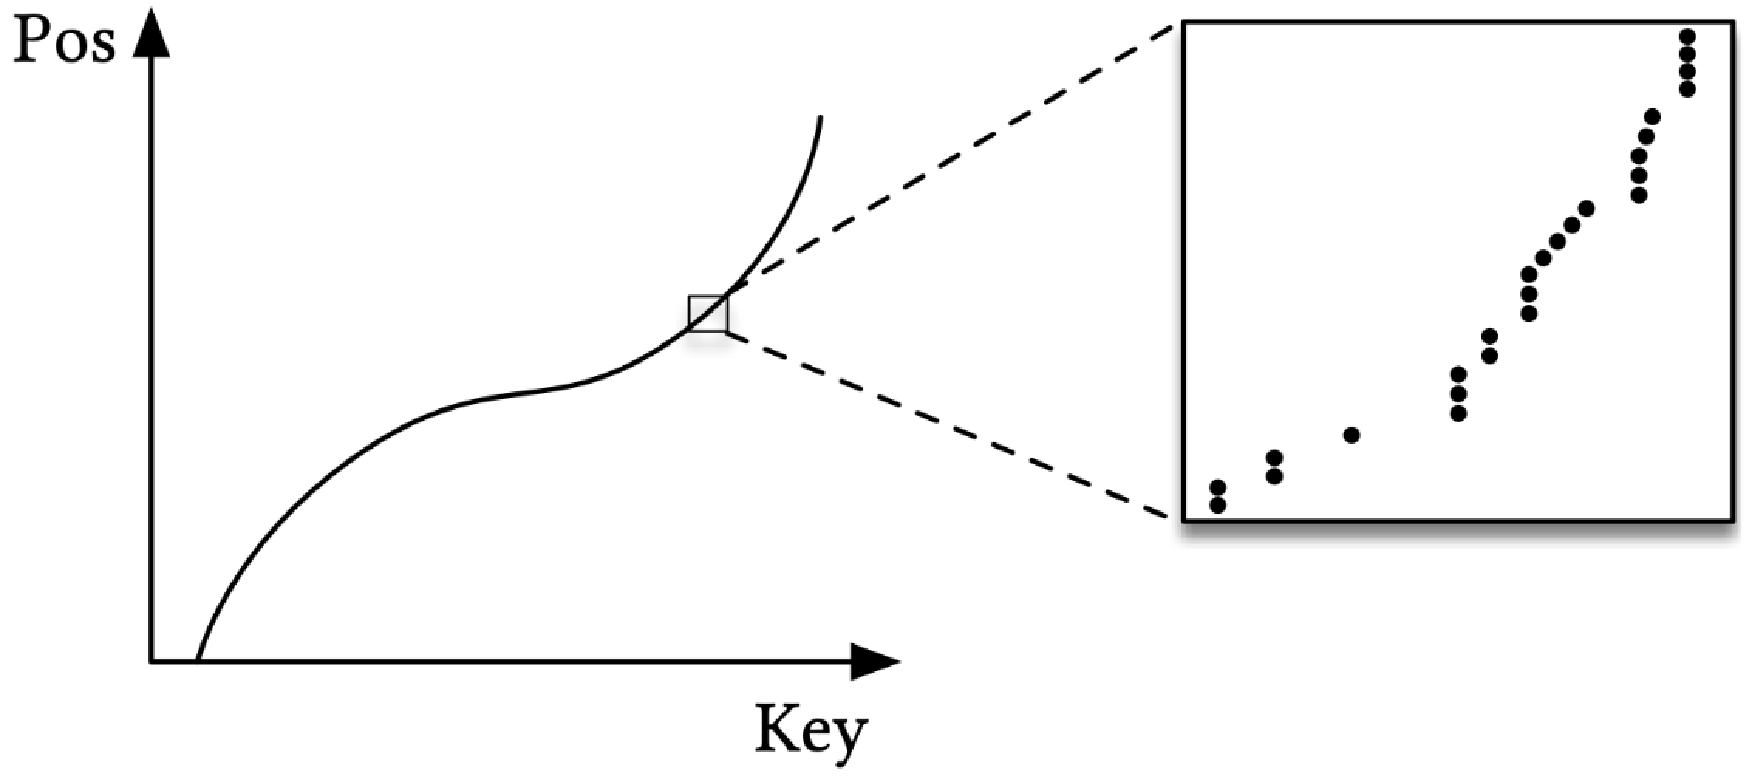
\includegraphics[width=0.8\textwidth]{graphs/introduction/cdf_assumptions}
\caption{The illustration of indexes as CDFs, originally from \cite{kraska2018case}}
\label{fig:indexes_as_cdf}
\end{figure}


Formally, we define the index of each record as $x$ and the corresponding location as $y$ and we represent the whole data as $(X, Y)$ pairs with the total number of pairs defined as $N$. We could then normalise the $Y$ into $\tilde{Y}\in[0,1]$ so that the $\tilde{y}$ represents the portion of the $y$ among the whole $Y$. With these definitions, we can then define a function $F:X\to \tilde{Y}$ that maps the index into the portion of the $y$. We have $y=F(x)* N$. As the output of this function can be considered as the probability of $X\leq x$, we can regard this function $F(x)$ as the cumulative distribution function (CDF) of $X$, i.e. $F(x)=\mathbb{P}(X\leq x)$. Now that $N$ is determined by the length of data records, we only need to learn such CDF and we called the learned CDF function as \textbf{learned index model}.

In Fig. \ref{fig:indexes_as_cdf}, we illustrate the relationship between the key and its position. The raw keys and their positions are illustrated in the zoomed-in view and the zoomed-out view presents a shape of the relation. In this figure, we present why the position can be regarded as a CDF: the position of a key is always the position of previous key plus $1$, i.e. the position describes how many keys are there before a certain key $x$. If we divide it by the total number of keys, we will have the result as the possibility of how many keys are smaller than the certain key $x$, i.e. $\mathbb{P}(X\leq x)$. The result is therefore the CDF of $X$.

\begin{mscexample}
	From the perspective of the distribution of data records, our previous example can be rephrased as following. Our data records are $(X, Y)$ pairs with a linear relation, i.e. $y=x, \forall y\in Y$. We are looking for a function $F$ such that $y=x=F(x)* N$, and hence we end up with $F(x)=\frac{1}{N}*x$. If we use this linear function $F(x)$ as the index model, then we could locate the data within $\mathcal{O}(1)$ time complexity and we only need to store the total number of records as the only parameter. Compared with B-Tree whose query complexity is $\mathcal{O}(\log n)$, the potential of using learned index to handle huge amount of data is enormous. 
\end{mscexample}

In order to ensure the learned index model to be the desired CDF, we need to make the following assumptions:

\begin{enumerate}
	\item All data records are stored statically. Hence we do not take insertion and deletion into consideration. If there is some insertion or deletion, then the total size of the data records, $N$, will be different. Therefore, if insertion or deletion are involved, we cannot calculate the position as we show above.
	\item All data records are sorted according to theirs keys $\boldsymbol{X}$. Only when the data records are sorted according to the keys, we can regard the index model as CDF, i.e. $F(x)=\mathbb{P}(X\leq x)$.
	\item For simplicity, we assume that our data records are stored in a continuous memory space. In other words, the indices of pages in this project is continuous integers and all the data records are loaded into memory.
\end{enumerate}